
\section{Introduction} % ----------------------------------------------
In the field of autonomous mobile robotics, there are many tasks that a robot has to perform in order to explore a new environment. One of these tasks is Simultaneous Localization And Mapping (SLAM), which is a well-known chicken-and-egg problem, where an accurate estimate of a robot pose is needed to create an accurate map, and vice versa an accurate map is needed to effectively estimate its pose. 

% -----------------------------------------------------------
%                                                           \
%                                                           \
% -----------------------------------------------------------

\subsection{Related work}\label{sec:related} % ----------------------------------------------
In the last decades, with the development of many new SLAM algorithms and techniques, there has been a growing need to find a common evaluation metric/framework. Many solutions are based either on manual evaluation \cite{balaguer2007visualEval}, or on other external information about the environment and robot operation. For example, a widely used metric that requires the latter is the Absolute Pose Error (APE), proposed by Kümmerle et al. in \cite{kummerle2009ATE}, which is divided into two sub-metrics: the Absolute Translational Error (ATE) and the Absolute Rotational Error (ARE). \textbf{Figure \ref{fig:APE_graphs}} shows how the ATE varies during the exploration of an environment, but for this work the main focus is on the average value calculated after the environment has been fully explored.

\begin{figure}[ht!]
    \centering
        \subfloat[ATE variation over time]{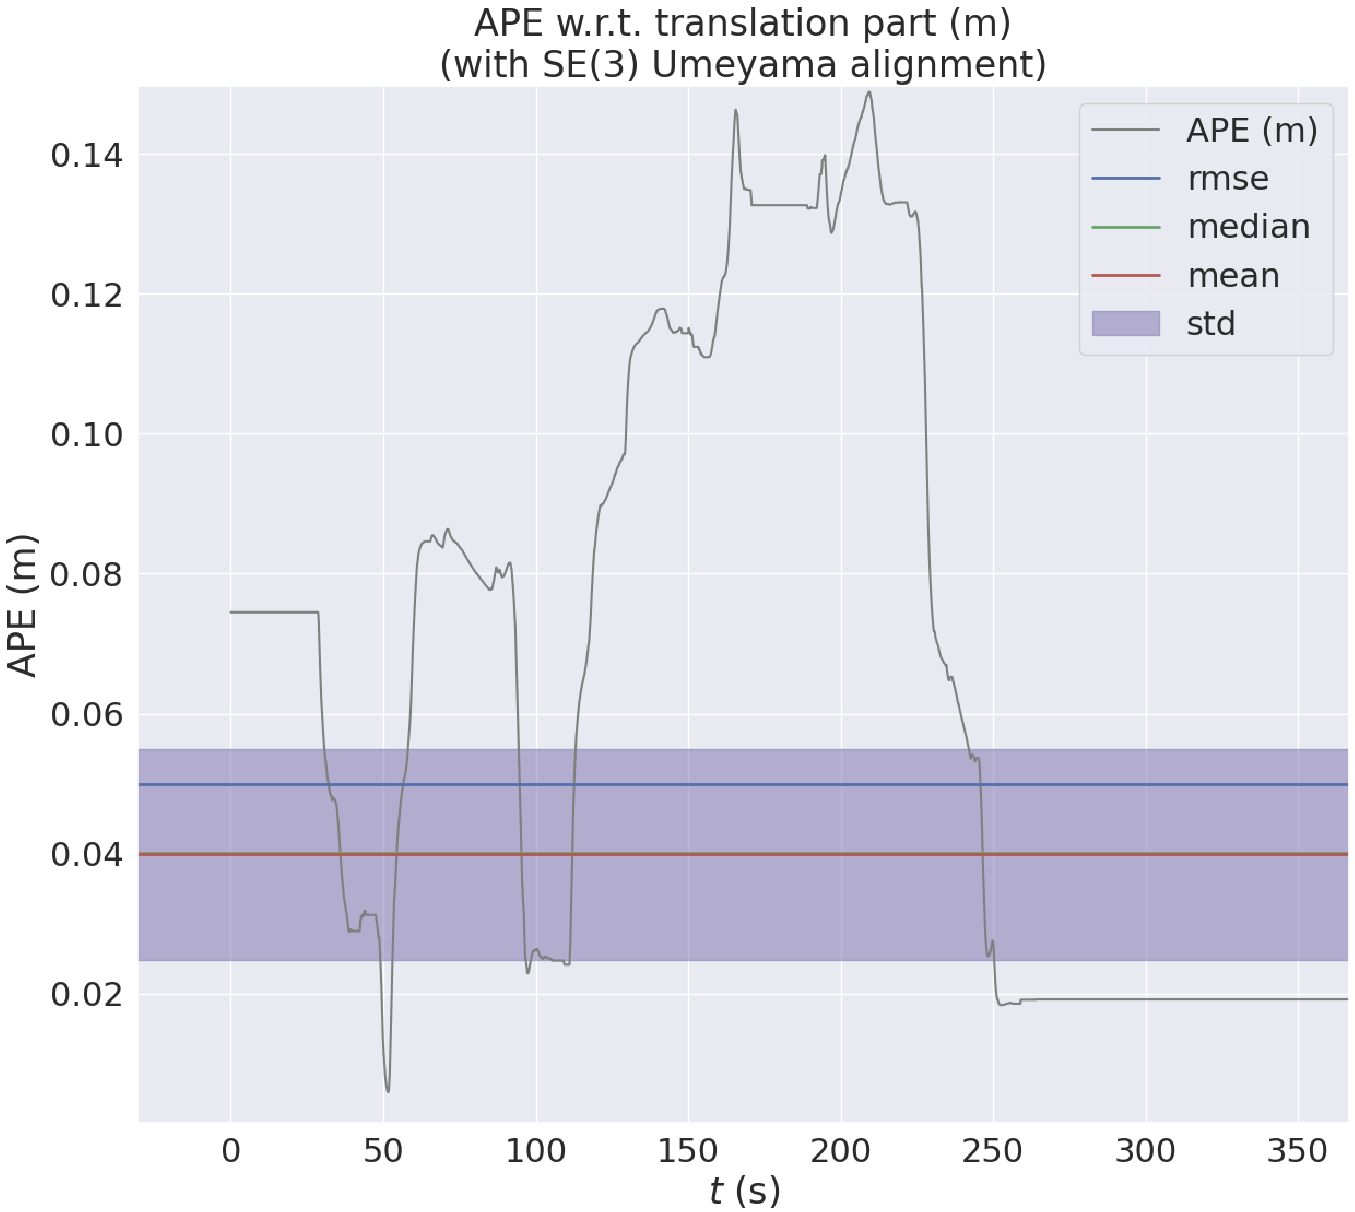
\includegraphics[width=.48\linewidth]{images/APE_graph.png}}\hfill
        \subfloat[ATE values over the map]{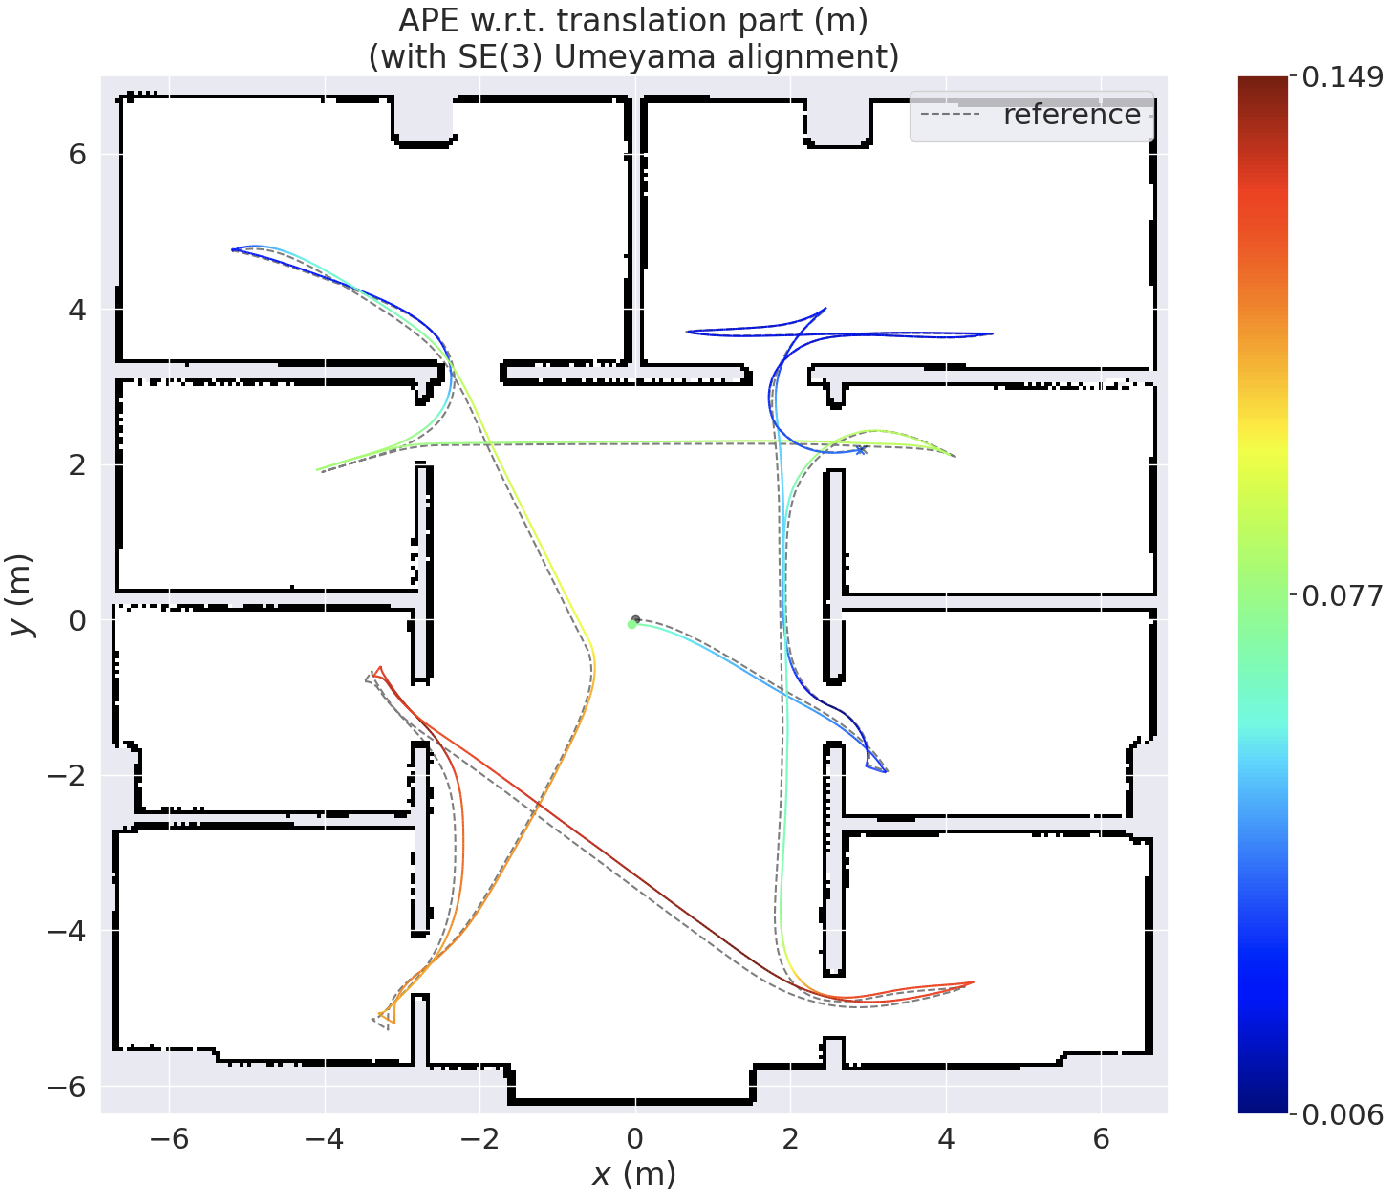
\includegraphics[width=.5\linewidth]{images/APE_map.png}}
    \caption{Visualizations of ATE variations during exploration, realized with \textit{evo}\protect\footnotemark.}\label{fig:APE_graphs}
    \end{figure}
\footnotetext{https://github.com/MichaelGrupp/evo}


\noindent
In order to compute ATE and ARE values after a robot has explored an environment, we need to compare all the pairs of key-points sampled from the estimated trajectory of the robot and its ground truth (GT) trajectory. Specifically, during exploration we sample $T$ poses, where each pose is a vector containing the position and orientation of the robot, and we build two sets $x_{1:T}$, $x_{1:T}^*$ that contain, respectively, the estimated and GT poses. \\
Next, we define $\delta_{i,j} = x_j\ominus x_i$ as the relative transformation\footnote{Which is a transformation matrix that describes a rigid transform.} that moves the robot from pose $x_i$ to $x_j$, and its counterpart $\delta_{i,j}^* = x_j^*\ominus x_j^*$. Then we define the $trans(\cdot)$ and $rot(\cdot)$ functions which extract, respectively, the translational component of a transform (i.e., a vector $z_{ij}\in\mathbb{R}^2$ representing the translation delta needed to move from pose i to j) and the rotational component (i.e., a vector $\theta_{ij}\in\mathbb{R}^2$ that expresses the angular deltas as Euler angles).
Finally, to compute the localization error we consider all sorted pairs of transformations $\{\delta_{i,j} : j < i, \forall i\in2\dots T\}$:

\begin{equation*}
    \begin{split}
        \centering
            \varepsilon(\delta) & = \varepsilon_t(\delta) + \varepsilon_r(\delta)\\
            & = \frac{1}{N}\sum_{i, j}trans(\delta_{i,j}\ominus\delta_{i,j}^*)+\frac{1}{N}\sum_{i, j}rot(\delta_{i,j}\ominus\delta_{i,j}^*)\\
            & = \frac{1}{N}\sum_{i, j}(||z_{ij} - z_{ij}^*||_2 + ||\theta_{ij} - \theta_{ij}^*||_2) \\
            & = \frac{2}{(T-1)^2}\sum_{i=2}^T\sum_{j=1}^{i-1}(||z_{ij} - z_{ij}^*||_2 + ||\theta_{ij} - \theta_{ij}^*||_2)\\
    \end{split}
\end{equation*}

\noindent
Note that these metrics are dependent on the availability of the GT data, which is easily obtained in simulated environments but extremely difficult to obtain when deploying a robot in the real world, as it would require an external system for accurately tracking its real position.\\

\noindent
To address the limitation of depending on the GT data, Luperto et al. in \cite{luperto2021predicting}, propose a method to perform an \textit{a-priori} prediction of the expected ATE and ARE, based on the geometric/topological characteristics of an indoor environment: using a feature extractor, described by Luperto et al. in \cite{luperto2019extracting}, a set of structural features is extracted from a floorplan, in order to represent each environment as a vector $v\in\mathbb{R}^k$, where $k$ is the number of distinct features.
Successively, each environment is explored by a simulated robot and, by collecting both GT and estimated trajectories, the corresponding ATE and ARE are computed and stored.

\noindent
Finally, two models are trained on this dataset:
\begin{itemize}
    \item \textbf{Linear model:} computed using linear regression.
    \item \textbf{Gaussian Process:} computed using an RBF kernel.
\end{itemize}

\begin{figure}[ht!]
    \centering
        \subfloat[KTH]{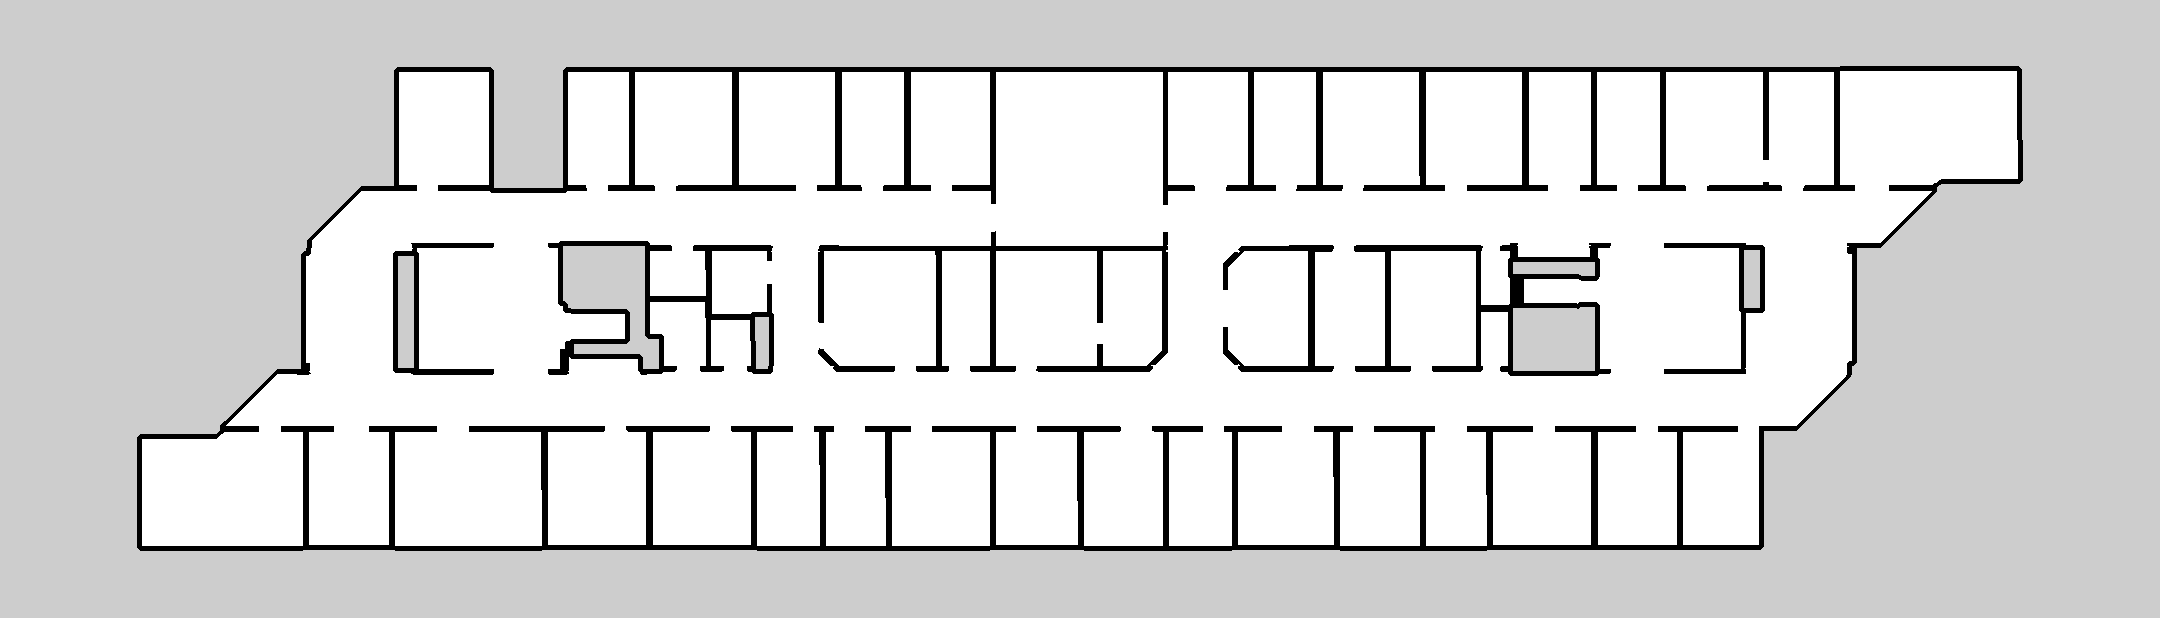
\includegraphics[width=.35\linewidth, angle=90]{images/50041171.png}}\hspace{.3in}
        \subfloat[MIT]{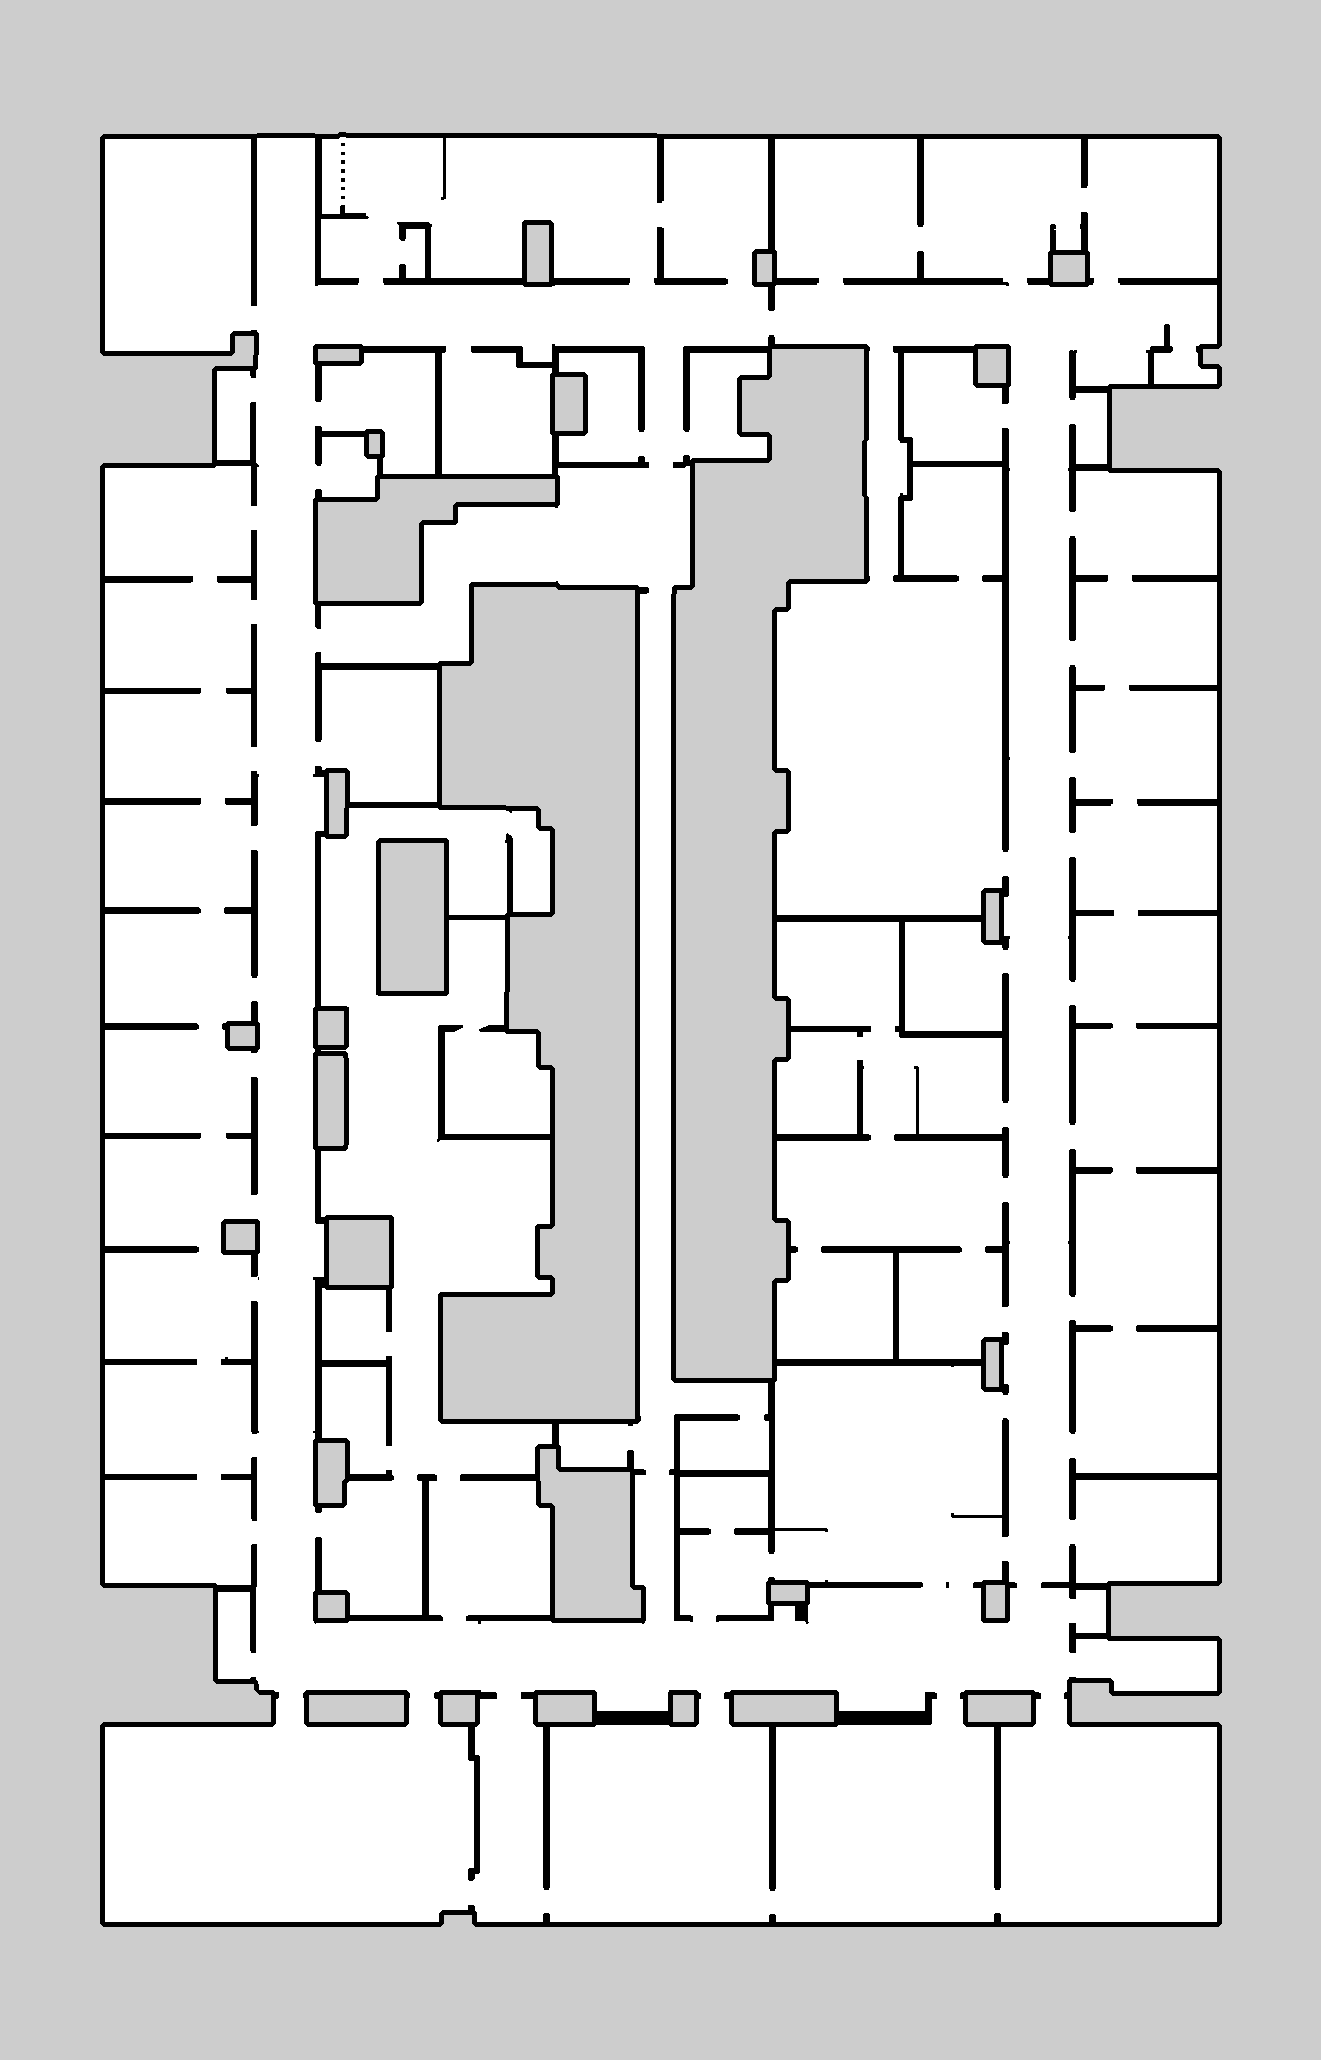
\includegraphics[height=.35\linewidth]{images/12-1.png}}\hspace{.3in}
        \subfloat[HouseExpo]{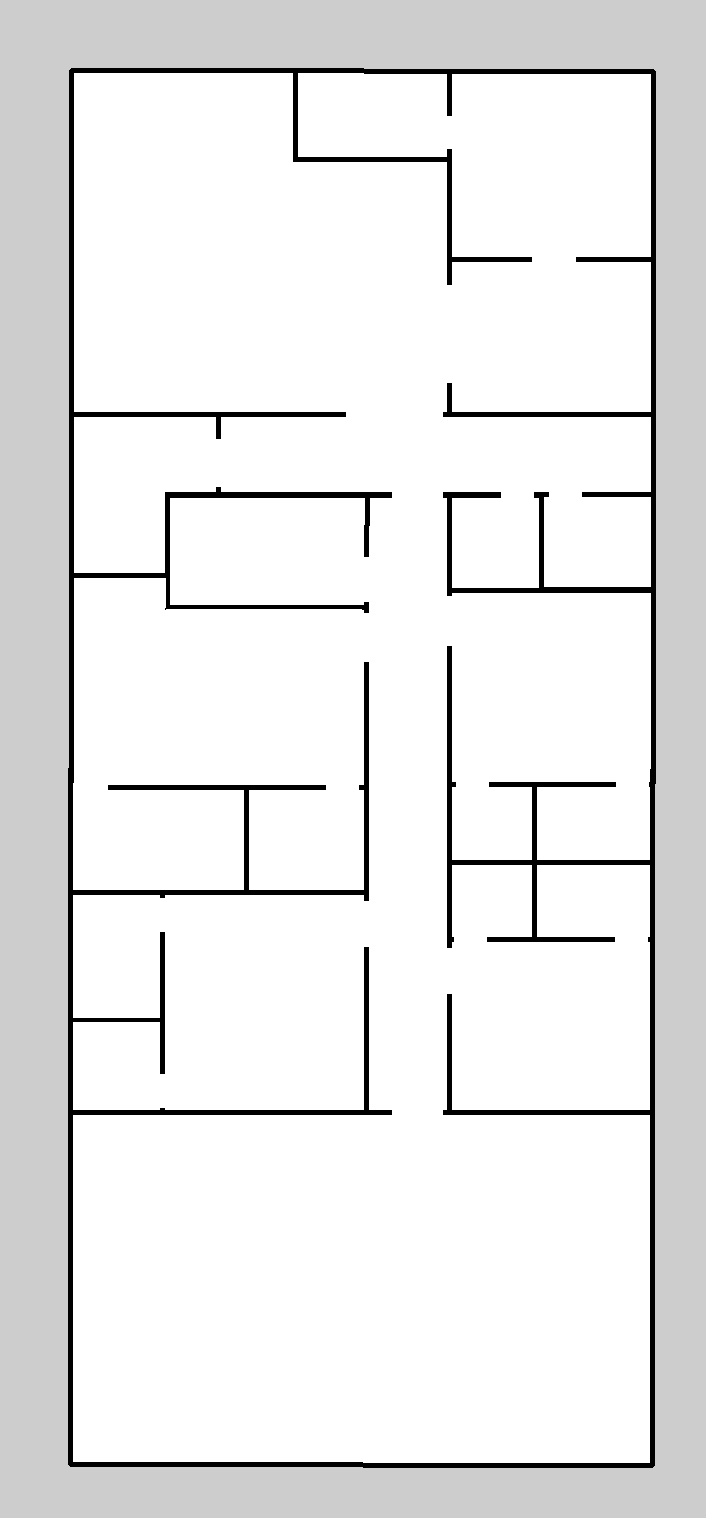
\includegraphics[height=.35\linewidth]{images/0a47882b40daf033e05e0b2dffafa6f7.png}}
    \caption{Example of floorplans from the datasets used in this work.}\label{fig:maxExample}
\end{figure}

% -----------------------------------------------------------
%                                                           \
%                                                           \
% -----------------------------------------------------------

\subsection{Task formulation} % -------------------------------------------------------
The goal of this project is to evaluate how a predictor, based on state-of-the-art convolutional neural networks (CNN), performs with respect to the aforementioned models. In particular, with the usage of a CNN, it is possible to delegate the feature extraction stage to the network itself, so that a floorplan's image can be fed directly to the model, without computing a set of hand-crafted features.  



\noindent
The dataset used in this work was collected for my Bachelor's thesis \textit{`Structural analysis of indoor environments for improving autonomous robotic tasks'}, and consists of floorplans and exploration data from three different sources: MIT campus \cite{whiting2006geometric}, KTH campus \cite{aydemir2012KTH}, and HouseExpo \cite{li2019houseexpo}. 
The joint dataset consists of 5933 floorplans, and contains both domestic and work/school environments, as shown in \textbf{Fig \ref{fig:maxExample}}.\\

\noindent
Each floorplan has associated three quantities: area ($m^2$), ATE ($m$), and ARE ($rad$); the floorplan image, together with the area, forms the input, while the labels consist of tuples containing the ATE and ARE values.

\noindent
More formally, the model $h$ we want to learn can be expressed as follows:
$$
    h: X \rightarrow Y\ ,\ X\in (Mat_{n \times n}\times\mathbb{R}),\ Y\in\mathbb{R}^2 
$$